% ============================================================
% SYNOPSIS
% GAP-AWARE RETRIEVAL FOR ITERATIVE RETRIEVAL-AUGMENTED
% GENERATION
%
% COMPILER:
% pdfLaTeX
%
% REQUIRED FILE:
% image1.png
% ============================================================

\documentclass[12pt,a4paper]{report}

% ============================================================
% FONT
% ============================================================

\usepackage{newtxtext,newtxmath}

% ============================================================
% PAGE SIZE AND MARGINS
% ============================================================

\usepackage[
    a4paper,
    top=0.66in,
    bottom=0.66in,
    left=0.78in,
    right=0.78in
]{geometry}

% ============================================================
% PACKAGES
% ============================================================

\usepackage{setspace}
\usepackage{graphicx}
\usepackage{array}
\usepackage{booktabs}
\usepackage{longtable}
\usepackage{tabularx}
\usepackage{ragged2e}
\usepackage{amsmath}
\usepackage{tikz}
\usepackage{eso-pic}
\usepackage{fancyhdr}
\usepackage{tocloft}
\usepackage{hyperref}
\usepackage{enumitem}
\usepackage{float}
\usepackage[table]{xcolor}
\usepackage{etoolbox}

\makeatletter
\patchcmd{\thebibliography}
  {\chapter*{\bibname}}
  {}
  {}
  {}
\makeatother
% ============================================================
% GENERAL FORMATTING
% ============================================================

\setlength{\parindent}{0pt}
\setlength{\parskip}{0pt}

\onehalfspacing

\hypersetup{
    colorlinks=false,
    hidelinks
}

% ============================================================
% PAGE BORDER
%
% Border is deliberately inside the physical page edge.
% It is applied to EVERY page.
% ============================================================

\AddToShipoutPictureBG{%
    \begin{tikzpicture}[remember picture,overlay]
        \draw[line width=0.5pt]
        ([xshift=0.30in,yshift=-0.30in]current page.north west)
        rectangle
        ([xshift=-0.30in,yshift=0.30in]current page.south east);
    \end{tikzpicture}%
}

% ============================================================
% HEADER / FOOTER
%
% Department name:
% TOP RIGHT
% SLIGHTLY ABOVE THE PAGE BORDER
%
% Page number:
% CENTERED
% SLIGHTLY RAISED FROM BOTTOM
% ============================================================

\pagestyle{fancy}

\fancyhf{}

% ------------------------------------------------------------
% Department name -- top right
% ------------------------------------------------------------

\fancyhead[R]{%
    \raisebox{0.22in}{%
        \fontsize{10}{12}\selectfont
        Department of Computer Engineering
    }%
}

% ------------------------------------------------------------
% Page number -- centered and raised
% ------------------------------------------------------------

\fancyfoot[C]{%
    \raisebox{0.18in}{%
        \fontsize{10}{12}\selectfont
        \thepage
    }%
}

% ------------------------------------------------------------
% Remove header/footer lines
% ------------------------------------------------------------

\renewcommand{\headrulewidth}{0pt}
\renewcommand{\footrulewidth}{0pt}

% ------------------------------------------------------------
% Header height
% ------------------------------------------------------------

\setlength{\headheight}{15pt}


% ============================================================
% CHAPTER-OPENING PAGES
%
% LaTeX normally changes chapter-opening pages to the
% "plain" style. Make it identical to the normal page style.
% ============================================================

\fancypagestyle{plain}{
    \fancyhf{}

    % Department name -- top right
    \fancyhead[R]{%
        \raisebox{0.22in}{%
            \fontsize{10}{12}\selectfont
            Department of Computer Engineering
        }%
    }

    % Page number -- centered and raised
    \fancyfoot[C]{%
        \raisebox{0.18in}{%
            \fontsize{10}{12}\selectfont
            \thepage
        }%
    }

    \renewcommand{\headrulewidth}{0pt}
    \renewcommand{\footrulewidth}{0pt}
}

% ============================================================
% TITLE COMMANDS
% ============================================================

\newcommand{\fronttitle}[1]{
    \begin{center}
        {\fontsize{18}{21}\selectfont\bfseries #1\par}
    \end{center}
    \vspace{0.12in}
}

\newcommand{\chaptertitle}[2]{
    \begin{center}
        {\fontsize{18}{21}\selectfont\bfseries CHAPTER #1\par}
        \vspace{0.10in}
        {\fontsize{18}{21}\selectfont\bfseries #2\par}
    \end{center}
    \vspace{0.12in}
}

% ============================================================
% DOCUMENT
% ============================================================

\begin{document}

% ============================================================
% PAGE 1
% TITLE PAGE
% ============================================================

\begin{titlepage}

\thispagestyle{empty}

\begin{center}

\vspace*{0.58in}

{\fontsize{16}{19}\selectfont\bfseries
Gap-Aware Retrieval (GAR):\par}

\vspace{0.08in}

{\fontsize{16}{19}\selectfont\bfseries
Adaptive Retrieval Using Information Gaps\par
and Existing Evidence\par}

\vspace{0.42in}

{\fontsize{12}{18}\selectfont
A Synopsis report submitted in\par}

\vspace{0.12in}

{\fontsize{12}{18}\selectfont
partial fulfillment of requirements for the degree of\par}

\vspace{0.12in}

{\fontsize{12}{18}\selectfont
Bachelor of Technology\par}

\vspace{0.10in}

{\fontsize{12}{18}\selectfont\bfseries\itshape
In\par}

\vspace{0.08in}

{\fontsize{12}{18}\selectfont
Computer Engineering\par}

\vspace{0.10in}

{\fontsize{12}{18}\selectfont\bfseries\itshape
By\par}

\vspace{0.08in}

{\fontsize{12}{18}\selectfont
Kunal Dahal (22CSEC17)\par
Aniket Manger (22CSEC23)\par
Suman Chettri (22CSEC44)\par}

\vspace{0.10in}

{\fontsize{12}{18}\selectfont\itshape
Under the supervision of\par}

\vspace{0.06in}

{\fontsize{14}{17}\selectfont\bfseries
Mr. Anmol Pandey\par}

\vspace{0.04in}

{\fontsize{12}{18}\selectfont
Assistant Professor\par}

\vspace{0.04in}

{\fontsize{12}{18}\selectfont
Computer Engineering Department\par}

\vspace{0.12in}

% ------------------------------------------------------------
% LOGO
% ------------------------------------------------------------


\includegraphics[width=0.82in]{image1.png}

\vspace{0.10in}

{\fontsize{14}{17}\selectfont\bfseries
Department Of Computer Engineering\par}

\vspace{0.04in}

{\fontsize{14}{17}\selectfont\bfseries
Sikkim Institute of Science and Technology\par}

\vspace{0.04in}

{\fontsize{14}{17}\selectfont\bfseries
(A constituent college of Sikkim University)\par}

\vspace{0.04in}

{\fontsize{14}{17}\selectfont\bfseries
2026\par}

\end{center}

\end{titlepage}

% ============================================================
% START ROMAN PAGE NUMBERING
% ============================================================

\pagenumbering{roman}
\setcounter{page}{1}

% ============================================================
% PAGE 2
% ABSTRACT
% ============================================================

\fronttitle{ABSTRACT}

\justifying

Retrieval-Augmented Generation (RAG) systems retrieve external information to support the generation of answers by large language models (LLMs). However, in complex and multi-hop questions, conventional retrieval methods may repeatedly retrieve information that is already available instead of focusing on the information that is still missing. This can limit the effectiveness of iterative retrieval.

This project is motivated by the MIGRES framework, which guides iterative retrieval using missing information. Based on the study of MIGRES and related retrieval approaches, this work will investigate the possibility of using the current information gap and previously collected evidence to guide document retrieval. The study will explore whether factors such as gap relevance, gap coverage, and evidence novelty can be considered to improve the selection of useful documents during iterative retrieval.

The proposed study will investigate whether explicitly incorporating the current information gap and previously collected evidence into the retrieval process can lead to more useful evidence selection in iterative RAG. As part of the work, a suitable retrieval strategy will be studied and developed within the MIGRES framework and will subsequently be evaluated against established retrieval approaches.

\vspace{0.10in}

\textbf{Keywords:}
Retrieval-Augmented Generation, Information Retrieval, MIGRES, Gap-Aware Retrieval, Information Gap, Multi-Hop Question Answering.
\clearpage


% ============================================================
% PAGE 3
% TABLE OF CONTENTS
% ============================================================

\fronttitle{TABLE OF CONTENTS}

\begin{center}

\renewcommand{\arraystretch}{1.45}

\makebox[\textwidth][c]{%
\begin{tabular}{|>{\centering\arraybackslash}p{0.55in}|
                >{\centering\arraybackslash}p{5.5in}|
                >{\centering\arraybackslash}p{0.55in}|}

\hline

\textbf{SL NO.} &
\textbf{TOPICS} &
\textbf{PAGE NO.} \\

\hline

&
ABSTRACT &
i \\

\hline

1. &
INTRODUCTION &
1 \\

\hline

2. &
LITERATURE SURVEY &
2--6 \\

\hline

3. &
PROBLEM DEFINITION &
7 \\

\hline

4. &
OBJECTIVES &
8 \\

\hline

5. &
APPLICATIONS &
9 \\

\hline

6. &
GANTT CHART &
10 \\

\hline

7. &
REFERENCES &
11 \\

\hline

\end{tabular}%
}

\end{center}

\clearpage


% ============================================================
% PAGE 4
% LIST OF TABLES AND FIGURES
% ============================================================

\fronttitle{LIST OF TABLES}

\begin{center}

\renewcommand{\arraystretch}{1.45}

\makebox[\textwidth][c]{%
\begin{tabular}{|>{\centering\arraybackslash}p{1.0in}|
                >{\centering\arraybackslash}p{4.8in}|
                >{\centering\arraybackslash}p{1.0in}|}

\hline

\textbf{TABLE NO.} &
\textbf{TITLE} &
\textbf{PAGE NO.} \\

\hline

2.1 & Literature Survey 1 & 2 \\

\hline

2.2 & Literature Survey 2 & 3 \\

\hline

2.3 & Literature Survey 3 & 4 \\

\hline

2.4 & Literature Survey 4 & 5 \\

\hline

2.5 & Literature Survey 5 & 6 \\

\hline

\end{tabular}%
}

\end{center}

\vspace{0.35in}

\fronttitle{LIST OF FIGURES}

\begin{center}

\renewcommand{\arraystretch}{1.45}

\makebox[\textwidth][c]{%
\begin{tabular}{|>{\centering\arraybackslash}p{1.0in}|
                >{\centering\arraybackslash}p{4.8in}|
                >{\centering\arraybackslash}p{1.0in}|}

\hline

\textbf{FIGURE NO.} &
\textbf{TITLE} &
\textbf{PAGE NO.} \\

\hline

6.1 & Gantt Chart & 10 \\

\hline

\end{tabular}%
}

\end{center}

\clearpage


% ============================================================
% CHAPTER 1
% INTRODUCTION
% ============================================================
\pagenumbering{arabic}
\setcounter{page}{1}
\addcontentsline{toc}{chapter}{1. INTRODUCTION}

\chaptertitle{1}{INTRODUCTION}

\justifying

Retrieval-Augmented Generation (RAG) combines information retrieval with large language models (LLMs) to improve answer generation using information from external documents. Instead of relying only on the knowledge stored in the model, RAG retrieves relevant information and provides it as context to the LLM. The quality of the retrieved information therefore has an important effect on the final answer.

Traditional retrieval methods mainly select documents based on their relevance to the given query. This can become challenging for complex and multi-hop questions, where the answer may require information from multiple documents. After one retrieval step, some information may already be available while other information may still be missing. In such cases, retrieving documents based only on the original query may result in repeated or less useful information.

The MIGRES framework addresses this issue by using missing information to guide iterative retrieval. After recovering and processing the evidence, MIGRES identifies what information is still missing and uses it to guide the next retrieval step \cite{wang2025migres}. This provides a useful direction for improving retrieval in multi-step question answering.

Recent research has also explored other ways to improve the usefulness of the retrieved information. Relevant Information Gain considers whether retrieved information provides useful new content rather than unnecessary repetition \cite{pickett2024better}. InfoGain-RAG similarly investigates document information gain for reranking and filtering retrieved documents \cite{wang2025infogain}. Other work has considered source reliability as an additional factor in RAG \cite{hwang2025reliability}, while ColBERTv2 provides an efficient late-interaction approach for document retrieval \cite{santhanam2022colbertv2}.

Based on the study of MIGRES and these related retrieval approaches, this project will investigate how iterative retrieval can make better use of the information that has already been collected and the information that is still required. In particular, the study will examine whether considering the current information gap and previously collected evidence can help in selecting more useful documents during subsequent retrieval steps.

As part of this investigation, the project will explore a retrieval strategy referred to as \textbf{Gap-Aware Retrieval (GAR)}. The study will examine the feasibility of considering factors such as gap relevance, gap coverage, and evidence novelty during document selection. The approach will be studied, developed, and evaluated during the subsequent stages of the project to determine its effectiveness in iterative RAG.

\clearpage


% ============================================================
% CHAPTER 2
% LITERATURE SURVEY
% ============================================================

\addcontentsline{toc}{chapter}{2. LITERATURE SURVEY}

\chaptertitle{2}{LITERATURE SURVEY}

\small

% ============================================================
% PAPER 1
% ============================================================

\begin{center}
\textbf{Table 2.1: Literature Survey 1}
\end{center}

\begin{longtable}{|p{1.25in}|p{5.15in}|}

\hline

\textbf{Name of paper} &
\textbf{LLMs Know What They Need: Leveraging a Missing Information Guided Framework to Empower Retrieval-Augmented Generation}
\\ \hline

\textbf{Authors} &
Keheng Wang, Feiyu Duan, Peiguang Li, Sirui Wang, and Xunliang Cai
\\ \hline

\textbf{Publication Details} &
Proceedings of the 31st International Conference on Computational Linguistics (COLING), 2025, pp. 2379--2400.
\\ \hline

\textbf{Research Findings} &
\begin{itemize}[
    leftmargin=0.18in,
    itemsep=0.05in,
    topsep=0pt,
    parsep=0pt
]
    \item The ability of LLMs to extract useful information from retrieved documents and identify information that is still missing is experimentally demonstrated.

    \item MIGRES is introduced as a Missing Information Guided Retrieve-Extraction-Solving framework, where the identified missing information is used to generate a targeted query for subsequent retrieval.

    \item Sentence-level reranking and filtering are introduced to remove irrelevant content from retrieved documents before useful information is extracted.
\end{itemize}
\\ \hline

\textbf{Research Gap} &
\begin{itemize}[
    leftmargin=0.18in,
    itemsep=0.05in,
    topsep=0pt,
    parsep=0pt
]
    \item Although MIGRES improves iterative retrieval, its performance still depends on the quality of the generated queries and the knowledge returned by the retriever.

    \item The framework can still encounter hard-negative passages that receive high relevance scores but do not provide useful information, which makes effective evidence selection challenging.
\end{itemize}
\\ \hline

\textbf{Relevance with Our Work} &
\begin{itemize}[
    leftmargin=0.18in,
    itemsep=0.05in,
    topsep=0pt,
    parsep=0pt
]
    \item MIGRES provides the base iterative RAG framework for investigating whether the retrieval stage can be further improved using the information available at each retrieval step.
\end{itemize}
\\ \hline

\end{longtable}

\clearpage


% ============================================================
% PAPER 2
% ============================================================

\begin{center}
\textbf{Table 2.2: Literature Survey 2}
\end{center}

\begin{longtable}{|p{1.25in}|p{5.15in}|}

\hline

\textbf{Name of paper} &
\textbf{Better RAG using Relevant Information Gain}
\\ \hline

\textbf{Authors} &
Marc Pickett, Jeremy Hartman, Ayan Kumar Bhowmick, Raquib-ul Alam, and Aditya Vempaty
\\ \hline

\textbf{Publication Details} &
arXiv preprint, 2024.
\\ \hline

\textbf{Research Findings} &
\begin{itemize}[
    leftmargin=0.18in,
    itemsep=0.05in,
    topsep=0pt,
    parsep=0pt
]
    \item The limited context window of RAG systems can cause redundant passages to occupy space that could otherwise be used for useful information.

    \item A Relevant Information Gain metric is introduced to measure the total information relevant to a query provided by a set of retrieved passages.

    \item The Dartboard retrieval method is developed using the proposed metric, allowing diverse passages to be selected without explicitly adding a separate diversity term.

    \item The method is evaluated on the Retrieval Augmented Generation Benchmark (RGB) and is reported to outperform existing retrieval approaches based on relevance and diversity.
\end{itemize}
\\ \hline

\textbf{Research Gap} &
\begin{itemize}[
    leftmargin=0.18in,
    itemsep=0.05in,
    topsep=0pt,
    parsep=0pt
]
    \item The proposed retrieval objective is defined for selecting a set of passages for a query, while the study does not specifically address how the retrieval objective should change when new evidence is collected through multiple retrieval steps.

    \item The evaluation is mainly conducted using the RGB benchmark, leaving the effectiveness of the approach in other iterative or multi-step retrieval settings open for further investigation.
\end{itemize}
\\ \hline

\textbf{Relevance with Our Work} &
\begin{itemize}[
    leftmargin=0.18in,
    itemsep=0.05in,
    topsep=0pt,
    parsep=0pt
]
    \item The paper provides a basis for considering the usefulness and redundancy of retrieved information when selecting documents, which is relevant to the retrieval problem being investigated in this project.
\end{itemize}
\\ \hline

\end{longtable}

\clearpage


% ============================================================
% PAPER 3
% ============================================================

\begin{center}
\textbf{Table 2.3: Literature Survey 3}
\end{center}

\begin{longtable}{|p{1.25in}|p{5.15in}|}

\hline

\textbf{Name of paper} &
\textbf{InfoGain-RAG: Boosting Retrieval-Augmented Generation through Document Information Gain-based Reranking and Filtering}
\\ \hline

\textbf{Authors} &
Zihan Wang, Zihan Liang, Zhou Shao, Yufei Ma, Huangyu Dai, Ben Chen, Lingtao Mao, Chenyi Lei, Yuqing Ding, and Han Li
\\ \hline

\textbf{Publication Details} &
Proceedings of the 2025 Conference on Empirical Methods in Natural Language Processing (EMNLP), 2025, pp. 7190--7204.
\\ \hline

\textbf{Research Findings} &
\begin{itemize}[
    leftmargin=0.18in,
    itemsep=0.05in,
    topsep=0pt,
    parsep=0pt
]
    \item Document Information Gain (DIG) is introduced to measure the contribution of an individual retrieved document to correct answer generation.

    \item DIG is calculated from the change in the LLM's generation confidence when a document is added to the context.

    \item InfoGain-RAG uses DIG scores to train a multi-task reranker that performs document filtering and ranking.

    \item Experiments across different RAG models and benchmarks show that the proposed method improves answer generation compared with several existing retrieval and reranking approaches.
\end{itemize}
\\ \hline

\textbf{Research Gap} &
\begin{itemize}[
    leftmargin=0.18in,
    itemsep=0.05in,
    topsep=0pt,
    parsep=0pt
]
    \item The current implementation is evaluated only on text-based retrieval tasks, while its application to other modalities such as visual or code information is left for future work.

    \item The DIG metric measures the contribution of a document to answer generation but cannot determine whether the information within that document is factually correct.

    \item The reranker size is limited by computational constraints, which may restrict the performance that could be obtained from larger models.
\end{itemize}
\\ \hline

\textbf{Relevance with Our Work} &
\begin{itemize}[
    leftmargin=0.18in,
    itemsep=0.05in,
    topsep=0pt,
    parsep=0pt
]
    \item The paper provides a useful basis for considering the contribution of retrieved documents when designing an improved document selection strategy.
\end{itemize}
\\ \hline

\end{longtable}

\clearpage


% ============================================================
% PAPER 4
% ============================================================

\begin{center}
\textbf{Table 2.4: Literature Survey 4}
\end{center}

\begin{longtable}{|p{1.25in}|p{5.15in}|}

\hline

\textbf{Name of paper} &
\textbf{Retrieval-Augmented Generation with Estimation of Source Reliability}
\\ \hline

\textbf{Authors} &
Jeongyeon Hwang, Junyoung Park, Hyejin Park, Dongwoo Kim, Sangdon Park, and Jungseul Ok
\\ \hline

\textbf{Publication Details} &
Proceedings of the 2025 Conference on Empirical Methods in Natural Language Processing (EMNLP), 2025, pp. 34279--34303.
\\ \hline

\textbf{Research Findings} &
\begin{itemize}[
    leftmargin=0.18in,
    itemsep=0.05in,
    topsep=0pt,
    parsep=0pt
]
    \item The effect of heterogeneous source reliability in multi-source RAG is investigated. It is shown that relying only on query-document relevance can allow information from unreliable sources to influence the generated answer.

    \item Reliability-Aware RAG (RA-RAG) is introduced, where source reliability is estimated by cross-checking information across multiple sources.

    \item Documents are selectively retrieved from highly reliable and relevant sources, and their information is aggregated using Weighted Majority Voting (WMV).

    \item Experiments show that RA-RAG improves performance over the compared baselines and remains effective as the number of information sources increases.
\end{itemize}
\\ \hline

\textbf{Research Gap} &
\begin{itemize}[
    leftmargin=0.18in,
    itemsep=0.05in,
    topsep=0pt,
    parsep=0pt
]
    \item Reliability estimation becomes more difficult when only a limited number of sources are available for cross-verification.

    \item The evaluation of real-world source reliability is mainly focused on news-related claims, while specialized topics with fewer available reference sources remain challenging.

    \item The reliability estimation process is performed in an offline setting and therefore requires periodic updates when the reliability of a source changes over time.
\end{itemize}
\\ \hline

\textbf{Relevance with Our Work} &
\begin{itemize}[
    leftmargin=0.18in,
    itemsep=0.05in,
    topsep=0pt,
    parsep=0pt
]
    \item The paper demonstrates that factors beyond query-document relevance can be incorporated into document selection, supporting the investigation of additional evidence-aware retrieval factors.
\end{itemize}
\\ \hline

\end{longtable}

\clearpage

% ============================================================
% PAPER 5
% ============================================================

\begin{center}
\textbf{Table 2.5: Literature Survey 5}
\end{center}

\begin{longtable}{|p{1.25in}|p{5.15in}|}

\hline

\textbf{Name of paper} &
\textbf{ColBERTv2: Effective and Efficient Retrieval via Lightweight Late Interaction}
\\ \hline

\textbf{Authors} &
Keshav Santhanam, Omar Khattab, Jon Saad-Falcon, Christopher Potts, and Matei Zaharia
\\ \hline

\textbf{Publication Details} &
Proceedings of the 2022 Conference of the North American Chapter of the Association for Computational Linguistics (NAACL), 2022, pp. 3715--3734.
\\ \hline

\textbf{Research Findings} &
\begin{itemize}[
    leftmargin=0.18in,
    itemsep=0.05in,
    topsep=0pt,
    parsep=0pt
]
    \item ColBERTv2 uses a late-interaction architecture in which query and document representations are independently encoded and compared at the token level.

    \item A residual compression mechanism is introduced to reduce the storage requirements of token-level document representations.

    \item Denoised supervision is used to improve the training of the retriever by reducing the effect of false negatives in the training data.

    \item ColBERTv2 achieves strong retrieval effectiveness while requiring substantially less storage than the original ColBERT model.
\end{itemize}
\\ \hline

\textbf{Research Gap} &
\begin{itemize}[
    leftmargin=0.18in,
    itemsep=0.05in,
    topsep=0pt,
    parsep=0pt
]
    \item The method still requires storing token-level representations for documents, which can result in considerable storage requirements for large collections.

    \item The retrieval architecture is designed primarily for efficient query-document matching, while the study does not investigate iterative retrieval with changing information requirements.
\end{itemize}
\\ \hline

\textbf{Relevance with Our Work} &
\begin{itemize}[
    leftmargin=0.18in,
    itemsep=0.05in,
    topsep=0pt,
    parsep=0pt
]
    \item ColBERTv2 provides an established neural retrieval method that can be considered as a retrieval baseline for evaluating an alternative retrieval strategy.
\end{itemize}
\\ \hline

\end{longtable}

\clearpage

% ============================================================
% CHAPTER 3
% PROBLEM DEFINITION
% ============================================================

\addcontentsline{toc}{chapter}{3. PROBLEM DEFINITION}

\chaptertitle{3}{PROBLEM DEFINITION}

\justifying

\begin{enumerate}[
    leftmargin=0.30in,
    itemsep=0.12in,
    parsep=0pt
]

\item
In iterative RAG, conventional retrieval may repeatedly retrieve documents that are relevant to the original query but contain information that has already been obtained. This can lead to redundant retrieval and reduce the usefulness of later retrieval steps.

\item
The information required to answer a multi-hop question can change as new evidence is collected. Existing retrieval methods may not sufficiently use the current missing information when selecting documents for the next retrieval step.

\item
Previously retrieved evidence can contain information that is already available to the system. A retrieval mechanism is therefore needed to consider the collected evidence along with the remaining information requirement when selecting further documents.

\item
The effectiveness of using the current information gap and previously collected evidence for iterative retrieval needs to be experimentally investigated and compared with existing retrieval approaches.

\end{enumerate}

\clearpage


% ============================================================
% CHAPTER 4
% OBJECTIVES
% ============================================================

\addcontentsline{toc}{chapter}{4. OBJECTIVES}

\chaptertitle{4}{OBJECTIVES}

\begin{enumerate}[
    leftmargin=0.30in,
    itemsep=0.12in,
    parsep=0pt
]

\item
To investigate methods for reducing redundant retrieval of information that has already been obtained.

\item
To study and incorporate the current missing information as a factor in selecting documents during iterative retrieval.

\item
To investigate how previously collected evidence can be considered when selecting documents for subsequent retrieval steps.

\item
To evaluate the effectiveness of the developed retrieval approach against existing retrieval methods using suitable retrieval and question-answering measures.

\end{enumerate}

\clearpage


% ============================================================
% CHAPTER 5
% APPLICATIONS
% ============================================================

\addcontentsline{toc}{chapter}{5. APPLICATIONS}

\chaptertitle{5}{APPLICATIONS}

\begin{enumerate}[
    leftmargin=0.30in,
    itemsep=0.12in
]

\item
\textbf{Multi-Hop Question Answering:}
The approach can be investigated for question-answering tasks that require information from multiple documents or retrieval steps.

\item
\textbf{Retrieval-Augmented Generation:}
The approach can be studied as a retrieval component for iterative RAG systems where additional information is retrieved as the answer is developed.

\item
\textbf{Research and Information Search:}
The approach may be useful for research-oriented systems where information is collected from multiple documents and previously retrieved evidence needs to be considered.

\item
\textbf{Evidence-Guided AI Systems:}
The approach may be applicable to AI systems that repeatedly retrieve external information and need to focus subsequent searches on information that is still required.

\end{enumerate}

\clearpage


% ============================================================
% CHAPTER 6
% PLANNING
% ============================================================

\addcontentsline{toc}{chapter}{6. GANTT CHART}

\chaptertitle{6}{GANTT CHART}

\begin{center}

\textbf{Figure 6.1: Gantt Chart}

\vspace{0.15in}

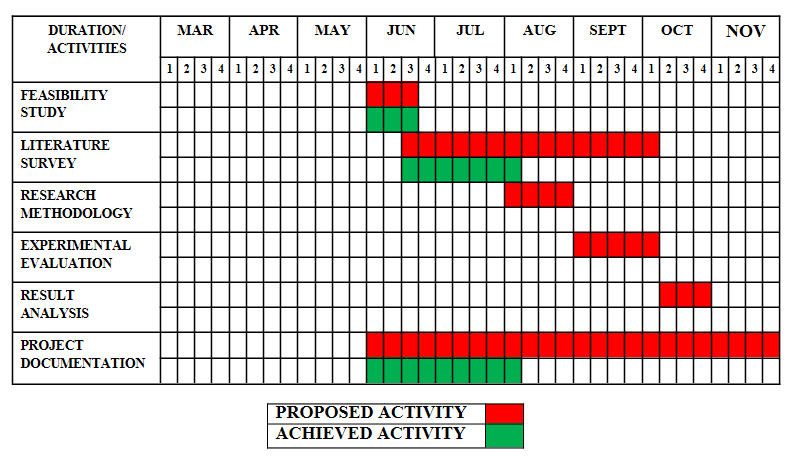
\includegraphics[width=0.95\textwidth]{gantt_chart.png}

\end{center}

\clearpage


% ============================================================
% CHAPTER 7
% REFERENCES
% ============================================================

\addcontentsline{toc}{chapter}{7. REFERENCES}

\chaptertitle{7}{REFERENCES}

\renewcommand{\bibname}{}

\bibliographystyle{IEEEtran}
\bibliography{citation}

\end{document}